% ══════════════════════════════════════════════════════════════
%  Rapport PFE — Météo Tunisie · Pipeline Big Data
%  ISIMS Sfax · Département ADBD · 2025-2026
% ══════════════════════════════════════════════════════════════
\documentclass[a4paper,12pt,oneside]{report}

% ─── Encodage et langue ───
\usepackage[utf8]{inputenc}
\usepackage[T1]{fontenc}
\usepackage[french]{babel}
\usepackage{csquotes}

% ─── Mise en page ───
\usepackage[top=2.5cm,bottom=2.5cm,left=3cm,right=2.5cm]{geometry}
\usepackage{setspace}
\onehalfspacing
\usepackage{fancyhdr}
\pagestyle{fancy}
\fancyhf{}
\fancyhead[L]{\leftmark}
\fancyhead[R]{\thepage}
\renewcommand{\headrulewidth}{0.4pt}

% ─── Graphiques et couleurs ───
\usepackage{graphicx}
\usepackage[dvipsnames,table]{xcolor}
\usepackage{float}
\usepackage{subcaption}
\usepackage{tikz}
\usetikzlibrary{shapes,arrows.meta,positioning,fit}

% ─── Tableaux ───
\usepackage{booktabs}
\usepackage{tabularx}
\usepackage{longtable}
\usepackage{multirow}
\usepackage{array}

% ─── Code source ───
\usepackage{listings}
\lstset{
  basicstyle=\ttfamily\small,
  backgroundcolor=\color{gray!8},
  frame=single,
  rulecolor=\color{gray!40},
  breaklines=true,
  numbers=left,
  numberstyle=\tiny\color{gray},
  keywordstyle=\color{blue!70!black}\bfseries,
  commentstyle=\color{green!50!black}\itshape,
  stringstyle=\color{red!60!black},
  showstringspaces=false,
  tabsize=2,
  captionpos=b
}

% ─── Liens et PDF ───
\usepackage[hidelinks]{hyperref}
\hypersetup{
  pdftitle={Météo Tunisie — Pipeline Big Data},
  pdfauthor={Équipe Projet ISIMS},
  pdfsubject={Rapport PFE},
}

% ─── Divers ───
\usepackage{amsmath,amssymb}
\usepackage{enumitem}
\usepackage{pifont}
\usepackage{tcolorbox}
\tcbuselibrary{skins,breakable}
\usepackage{caption}
\usepackage{url}

% ─── Commandes personnalisées ───
\newcommand{\imgplaceholder}[2]{%
  \begin{tcolorbox}[colback=blue!5,colframe=blue!40,title=#1]
    \centering\itshape #2\\[6pt]
    \texttt{$\rightarrow$ Insérer la capture ici}
  \end{tcolorbox}
}

% ══════════════════════════════════════════════════════════════
\begin{document}

% ─────────────────────────────────────────
%  PAGE DE GARDE
% ─────────────────────────────────────────
\begin{titlepage}
\centering
\vspace*{1cm}

% Logo université
% \includegraphics[width=4cm]{figures/logo_isims.png}
\imgplaceholder{Logo}{Logo ISIMS Sfax}

\vspace{0.5cm}
{\large \textbf{Université de Sfax}}\\[4pt]
{\large Institut Supérieur d'Informatique et de Multimédia de Sfax}\\[4pt]
{\large Département ADBD}\\[1.5cm]

{\Large \textbf{RAPPORT DE PROJET}}\\[0.3cm]
{\large Année universitaire 2025--2026}\\[1.5cm]

\rule{\textwidth}{1.5pt}\\[0.4cm]
{\LARGE \textbf{Météo Tunisie}}\\[0.2cm]
{\Large Pipeline Big Data de Collecte, Analyse et\\Visualisation des Données Météorologiques}\\[0.4cm]
\rule{\textwidth}{1.5pt}\\[2cm]

\begin{minipage}[t]{0.45\textwidth}
\textbf{Réalisé par :}\\
Mohamed Chaari\\
Yessine [Nom]\\
Moataz [Nom]\\
Brahim [Nom]
\end{minipage}
\hfill
\begin{minipage}[t]{0.45\textwidth}
\raggedleft
\textbf{Encadré par :}\\
Mme Nesrine [Nom]
\end{minipage}

\vfill
{\large Sfax, 2025--2026}
\end{titlepage}

% ─────────────────────────────────────────
%  DÉDICACES
% ─────────────────────────────────────────
\chapter*{Dédicaces}
\addcontentsline{toc}{chapter}{Dédicaces}
\thispagestyle{empty}
\vspace*{3cm}
\begin{center}
\textit{À nos familles,\\
qui nous ont soutenus tout au long de ce parcours.\\[1cm]
À nos enseignants,\\
pour leur patience et leur dévouement.\\[1cm]
À tous ceux qui ont contribué,\\
de près ou de loin, à la réalisation de ce projet.}
\end{center}
\newpage

% ─────────────────────────────────────────
%  REMERCIEMENTS
% ─────────────────────────────────────────
\chapter*{Remerciements}
\addcontentsline{toc}{chapter}{Remerciements}

Nous tenons à exprimer nos sincères remerciements à notre encadrante, \textbf{Mme Nesrine [Nom]}, pour son accompagnement, ses conseils précieux et sa disponibilité tout au long de ce projet.

Nous remercions également l'ensemble du corps enseignant du département ADBD de l'ISIMS de Sfax pour la formation de qualité qu'ils nous ont dispensée.

Enfin, nous adressons nos remerciements à toutes les personnes qui ont contribué, de près ou de loin, à la réalisation de ce travail.

\newpage

% ─────────────────────────────────────────
%  RÉSUMÉ
% ─────────────────────────────────────────
\chapter*{Résumé}
\addcontentsline{toc}{chapter}{Résumé}

\textbf{Français :}\\
Ce projet porte sur la conception et le développement d'une plateforme Big Data dédiée à la collecte, l'analyse et la visualisation des données météorologiques de 221 villes tunisiennes. L'architecture s'appuie sur un pipeline de streaming en temps réel utilisant Apache Kafka (Aiven) pour l'ingestion, Supabase (PostgreSQL) pour le stockage, Apache Airflow pour l'orchestration des analyses, et une API REST FastAPI pour l'exposition des données. Le système couvre l'historique météorologique de 2020 à 2024, l'ingestion temps réel toutes les 15 minutes, ainsi que des analyses avancées incluant la détection de pics thermiques, les corrélations saisonnières et les tendances annuelles.

\vspace{0.8cm}
\textbf{English:}\\
This project focuses on designing and developing a Big Data platform for collecting, analyzing, and visualizing meteorological data from 221 Tunisian cities. The architecture relies on a real-time streaming pipeline using Apache Kafka (Aiven) for ingestion, Supabase (PostgreSQL) for storage, Apache Airflow for analysis orchestration, and a FastAPI REST API for data exposure. The system covers the weather history from 2020 to 2024, real-time ingestion every 15 minutes, and advanced analytics including thermal peak detection, seasonal correlations, and annual trends.

\newpage

% ─────────────────────────────────────────
%  LISTE DES ABRÉVIATIONS
% ─────────────────────────────────────────
\chapter*{Liste des Abréviations}
\addcontentsline{toc}{chapter}{Liste des Abréviations}

\begin{tabularx}{\textwidth}{lX}
\toprule
\textbf{Abréviation} & \textbf{Signification} \\
\midrule
API     & Application Programming Interface \\
ADBD    & Administration des Bases de Données \\
DAG     & Directed Acyclic Graph \\
DB      & Database (Base de données) \\
E2E     & End-to-End \\
JWT     & JSON Web Token \\
KPI     & Key Performance Indicator \\
OWM     & OpenWeatherMap \\
PaaS    & Platform as a Service \\
REST    & Representational State Transfer \\
SaaS    & Software as a Service \\
SQL     & Structured Query Language \\
SSL     & Secure Sockets Layer \\
UI/UX   & User Interface / User Experience \\
US      & User Story \\
\bottomrule
\end{tabularx}

\newpage

% ─────────────────────────────────────────
%  TABLES
% ─────────────────────────────────────────
\tableofcontents
\newpage
\listoffigures
\addcontentsline{toc}{chapter}{Liste des Figures}
\newpage
\listoftables
\addcontentsline{toc}{chapter}{Liste des Tableaux}
\newpage

% ══════════════════════════════════════════════════════════════
%  CHAPITRES
% ══════════════════════════════════════════════════════════════
% ══════════════════════════════════════════
%  CHAPITRE 1 — INTRODUCTION GÉNÉRALE
% ══════════════════════════════════════════
\chapter{Introduction Générale}

\section{Contexte et motivation}
La météorologie joue un rôle crucial dans plusieurs secteurs comme l'agriculture, le tourisme ou la gestion des risques. Actuellement, l'accès à des données météorologiques historiques et en temps réel de manière centralisée reste complexe en Tunisie.

Ce projet vise à résoudre ce problème en utilisant les technologies du Big Data. L'objectif est de créer une plateforme centralisée capable de collecter, traiter et analyser les données météorologiques de plusieurs villes tunisiennes.

\section{Problématique}
Le défi principal de ce projet est de répondre à la question suivante :
Comment concevoir et déployer une plateforme complète capable de :
\begin{itemize}
  \item Collecter des données météo fiables pour l'ensemble des villes tunisiennes ?
  \item Traiter ces flux de données en temps réel ?
  \item Analyser ces données pour en extraire des statistiques utiles ?
  \item Présenter les résultats sur une interface web simple et interactive ?
\end{itemize}

\section{Objectifs du projet}
Pour répondre à cette problématique, nous avons défini les objectifs suivants :
\begin{enumerate}
  \item \textbf{Collecte de données :} Intégrer des APIs météorologiques pour récupérer l'historique et les données actuelles de 221 villes.
  \item \textbf{Infrastructure Big Data :} Mettre en place un système de streaming (Kafka) et une base de données robuste (Supabase).
  \item \textbf{Orchestration :} Automatiser les analyses et la détection d'alertes avec Apache Airflow.
  \item \textbf{Visualisation :} Développer un tableau de bord (Dashboard) interactif pour afficher les données.
\end{enumerate}

\section{Structure du rapport}
Ce rapport s'organise de la manière suivante :
\begin{itemize}
  \item \textbf{Chapitre 2} : Présente l'état de l'art et les outils utilisés.
  \item \textbf{Chapitre 3} : Détaille la méthodologie de travail Scrum.
  \item \textbf{Chapitre 4} : Décrit le Sprint 1 (Infrastructure et Flux temps réel).
  \item \textbf{Chapitre 5} : Décrit le Sprint 2 (Analyses statistiques et Déploiement).
  \item \textbf{Chapitre 6} : Présente les tests globaux et la validation du système.
\end{itemize}

% ══════════════════════════════════════════
%  CHAPITRE 2 — ÉTAT DE L'ART
% ══════════════════════════════════════════
\chapter{État de l'Art}

\section{Systèmes météorologiques existants}
Il existe de nombreuses sources de données météorologiques. Pour ce projet, nous avons comparé plusieurs solutions :
\begin{itemize}
    \item \textbf{Open-Meteo} : Une API gratuite offrant un historique riche sans clé d'accès (Choix principal).
    \item \textbf{OpenWeatherMap} : Une API très populaire, utile pour les données en temps réel (Choix secondaire).
    \item \textbf{Météo-France / INM Tunisie} : Données précises mais accès souvent payant ou limité.
\end{itemize}

\section{Technologies Big Data choisies}
Pour traiter ce grand volume de données, nous avons sélectionné les technologies suivantes :
\begin{itemize}
    \item \textbf{Apache Kafka} : Utilisé pour recevoir les données en continu (streaming) sans surcharger le système.
    \item \textbf{Apache Airflow} : Permet d'automatiser et de planifier les calculs tous les jours.
    \item \textbf{PostgreSQL (Supabase)} : Une base de données cloud très performante pour stocker tout l'historique météo de manière sécurisée.
\end{itemize}

\section{Comparaison avec les solutions existantes}
Comparé à d'autres applications grand public, notre plateforme se démarque par :
\begin{itemize}
    \item \textbf{Une spécialisation locale} : Une couverture complète des 221 villes tunisiennes.
    \item \textbf{Des analyses sur-mesure} : La plateforme ne se contente pas d'afficher le temps qu'il fait, elle calcule des statistiques et alerte automatiquement sur les pics de chaleur.
    \item \textbf{Une architecture moderne} : L'utilisation de technologies Big Data permet au système de traiter énormément de données très rapidement.
\end{itemize}

\section{Positionnement de notre solution}
Notre projet se positionne comme un outil complet, allant de la collecte des données brutes à l'analyse avancée, le tout centralisé sur un tableau de bord pensé pour des utilisateurs recherchant des informations météorologiques précises sur la Tunisie.

% ══════════════════════════════════════════
%  CHAPITRE 3 — MÉTHODOLOGIE SCRUM
% ══════════════════════════════════════════
\chapter{Méthodologie Scrum et Spécifications Globales}

\section{Présentation de la démarche Scrum}
Le projet a été mené selon la méthodologie agile \textbf{Scrum}, structurée en deux sprints de durée égale. Cette approche itérative nous a permis de livrer un incrément fonctionnel à chaque fin de sprint et d'adapter les priorités en fonction des retours.

\begin{figure}[H]
\centering
\imgplaceholder{Figure~\ref{fig:scrum_cycle} — Cycle Scrum}{Diagramme illustrant le cycle Scrum avec Product Backlog, Sprint Planning, Daily Scrum, Sprint Review et Retrospective}
\caption{Cycle de développement Scrum appliqué au projet}
\label{fig:scrum_cycle}
\end{figure}

\textbf{Rôles~:}
\begin{itemize}
  \item \textbf{Product Owner}~: Mme Nesrine [Nom] (encadrante)
  \item \textbf{Scrum Master}~: Mohamed Chaari
  \item \textbf{Équipe de développement}~: Mohamed, Yessine, Moataz, Brahim
\end{itemize}

\section{Identification des acteurs}

\begin{table}[H]
\centering
\caption{Acteurs du système}
\label{tab:acteurs}
\begin{tabularx}{\textwidth}{lX}
\toprule
\textbf{Acteur} & \textbf{Description} \\
\midrule
Utilisateur    & Consulte le dashboard, les prévisions et les analyses \\
Administrateur & Gère l'infrastructure Cloud et les configurations \\
Analyste       & Consulte les analyses statistiques avancées et les alertes \\
Système        & Exécute automatiquement les pipelines et les DAGs \\
\bottomrule
\end{tabularx}
\end{table}

\section{Besoins fonctionnels et non fonctionnels globaux}

\subsection{Besoins fonctionnels}
\begin{enumerate}
  \item Collecter les données météo historiques (2020--2024) et temps réel pour 221 villes.
  \item Ingérer les données via un système de streaming fiable (Kafka).
  \item Stocker les données dans une base PostgreSQL Cloud (Supabase).
  \item Orchestrer les analyses automatisées (moyennes, corrélations, pics, tendances).
  \item Exposer les données via une API REST documentée.
  \item Afficher les résultats dans un dashboard interactif avec cartes et graphiques.
\end{enumerate}

\subsection{Besoins non fonctionnels}
\begin{itemize}
  \item \textbf{Performance}~: Ingestion de $>$200 enregistrements/batch sans perte.
  \item \textbf{Disponibilité}~: Infrastructure Cloud avec haute disponibilité (Supabase, Aiven).
  \item \textbf{Sécurité}~: Connexions SSL pour Kafka, mots de passe chiffrés.
  \item \textbf{Maintenabilité}~: Code modulaire avec tests unitaires ($>$100 tests).
  \item \textbf{Scalabilité}~: Architecture découplée permettant l'ajout de nouvelles villes ou sources.
\end{itemize}

\section{Diagramme de cas d'utilisation global}

\begin{figure}[H]
\centering
\imgplaceholder{Figure~\ref{fig:uc_global} — Diagramme de cas d'utilisation global}{Diagramme UML montrant les 4 acteurs (Utilisateur, Administrateur, Analyste, Système) et les cas d'utilisation principaux~: Consulter Dashboard, Voir Prévisions, Analyser Tendances, Recevoir Alertes, Configurer Infrastructure, Exécuter Pipeline}
\caption{Diagramme de cas d'utilisation global}
\label{fig:uc_global}
\end{figure}

\section{Product Backlog complet}

\begin{table}[H]
\centering
\caption{Product Backlog — Liste des User Stories}
\label{tab:backlog}
\begin{tabularx}{\textwidth}{clXcc}
\toprule
\textbf{US} & \textbf{Sprint} & \textbf{Description} & \textbf{Priorité} & \textbf{Points} \\
\midrule
US1 & S1 & Configuration de Supabase et Aiven            & Haute & 8 \\
US2 & S1 & Producer live et Consumer vers la DB            & Haute & 13 \\
US3 & S1 & Endpoints API /summary et /forecast             & Moyenne & 8 \\
US4 & S1 & Authentification JWT                             & Moyenne & 5 \\
US5 & S1 & Dashboard et graphiques de prévisions            & Haute & 13 \\
US6 & S1 & Validation des flux et plan de test              & Basse & 3 \\
\midrule
US7 & S2 & DAGs Airflow (moyennes, corrélations)            & Haute & 13 \\
US8 & S2 & Détection de pics (canicule, tempêtes)            & Haute & 8 \\
US9 & S2 & Documentation, monitoring et livraison finale     & Moyenne & 5 \\
\bottomrule
\end{tabularx}
\end{table}

\section{Architecture globale du système}

\begin{figure}[H]
\centering
\imgplaceholder{Figure~\ref{fig:archi_globale} — Architecture globale du pipeline}{Diagramme d'architecture montrant~: APIs Météo $\rightarrow$ Producer Python $\rightarrow$ Aiven Kafka $\rightarrow$ Consumer Python $\rightarrow$ Supabase PostgreSQL $\rightarrow$ Airflow DAGs $\rightarrow$ FastAPI $\rightarrow$ Dashboard Frontend}
\caption{Architecture globale du système Météo Tunisie}
\label{fig:archi_globale}
\end{figure}

\section{Planification des Sprints}

\begin{table}[H]
\centering
\caption{Répartition des Sprints}
\label{tab:sprints}
\begin{tabularx}{\textwidth}{lXl}
\toprule
\textbf{Sprint} & \textbf{Objectif} & \textbf{User Stories} \\
\midrule
Sprint 1 & Infrastructure Cloud et Flux Temps Réel    & US1 à US6 \\
Sprint 2 & Analyses Avancées, Alertes et Déploiement   & US7 à US9 \\
\bottomrule
\end{tabularx}
\end{table}

% ══════════════════════════════════════════
%  CHAPITRE 4 — SPRINT 1
% ══════════════════════════════════════════
\chapter{Sprint 1~: Infrastructure Cloud et Flux Temps Réel}

\section{Introduction}
Le premier sprint marque le lancement technique du projet. L'objectif est de mettre en place une architecture robuste et évolutive en s'appuyant sur des services Cloud (SaaS/PaaS). Cette phase se concentre sur la création de la base de données sur Supabase, la configuration du broker de messages Kafka via Aiven, et le développement du socle de l'API permettant de faire circuler les premières données météorologiques de bout en bout.

\section{Objectif du Sprint et Sprint Backlog}

\subsection{Objectif attendu}
Déployer l'infrastructure Cloud, charger l'historique météo (2020--2024) pour les 221 villes, et activer le flux d'ingestion en temps réel pour alimenter un tableau de bord dynamique et sécurisé.

\subsection{Sprint Backlog}

\begin{table}[H]
\centering
\caption{Sprint Backlog — Sprint 1}
\label{tab:sprint1_backlog}
\begin{tabularx}{\textwidth}{clX}
\toprule
\textbf{US} & \textbf{Catégorie} & \textbf{Description} \\
\midrule
US1 & Infrastructure & Configuration de Supabase (PostgreSQL) et Aiven (Kafka) \\
US2 & Ingestion      & Développement du Producer live et du Consumer vers la DB \\
US3 & API Core       & Création des endpoints \texttt{/summary} et \texttt{/forecast} \\
US4 & Sécurité       & Mise en place de l'authentification JWT \\
US5 & UI/UX          & Intégration du Dashboard et des graphiques de prévisions \\
US6 & Qualité        & Validation des flux et rédaction du plan de test \\
\bottomrule
\end{tabularx}
\end{table}

\section{Analyse et Spécification}

\subsection{Diagramme de cas d'utilisation du Sprint 1}

\begin{figure}[H]
\centering
\imgplaceholder{Figure~\ref{fig:uc_sprint1} — Cas d'utilisation Sprint 1}{Diagramme UML avec acteurs Administrateur, Système et Utilisateur. Cas~: Configurer Infrastructure, Ingérer Données Historiques, Consulter Dashboard, S'authentifier}
\caption{Diagramme de cas d'utilisation — Sprint 1}
\label{fig:uc_sprint1}
\end{figure}

\subsection{Description textuelle des cas d'utilisation}

\begin{table}[H]
\centering
\caption{Cas d'utilisation — Consulter les données temps réel (US5)}
\label{tab:uc_dashboard}
\begin{tabularx}{\textwidth}{lX}
\toprule
\textbf{Élément} & \textbf{Description} \\
\midrule
Acteur         & Utilisateur \\
Pré-conditions & L'utilisateur est authentifié ; les flux Aiven/Supabase sont actifs \\
Scénario nominal & 1. L'utilisateur accède au dashboard \\
               & 2. Le système appelle l'API \texttt{/api/dashboard/summary} \\
               & 3. L'interface affiche les KPIs météo mis à jour \\
Post-conditions & Les données sont affichées avec la dernière mise à jour \\
\bottomrule
\end{tabularx}
\end{table}

\begin{table}[H]
\centering
\caption{Cas d'utilisation — S'authentifier (US4)}
\label{tab:uc_auth}
\begin{tabularx}{\textwidth}{lX}
\toprule
\textbf{Élément} & \textbf{Description} \\
\midrule
Acteur         & Utilisateur \\
Scénario nominal & 1. Saisie des identifiants (email + mot de passe) \\
               & 2. Vérification dans la table \texttt{users} de Supabase \\
               & 3. Génération et renvoi d'un token JWT \\
Scénario alternatif & Identifiants incorrects $\rightarrow$ message d'erreur \\
\bottomrule
\end{tabularx}
\end{table}

\section{Conception}

\subsection{Conception de la base de données}

\begin{figure}[H]
\centering
\imgplaceholder{Figure~\ref{fig:schema_db} — Schéma relationnel Supabase}{Schéma montrant les 8 tables~: weather\_historical, weather\_current, weather\_forecast, monthly\_averages, correlations, temperature\_peaks, annual\_stats, pipeline\_runs avec leurs relations et clés}
\caption{Schéma relationnel de la base de données Supabase}
\label{fig:schema_db}
\end{figure}

\subsection{Dictionnaire de données}

\begin{table}[H]
\centering
\caption{Dictionnaire de données — Table \texttt{weather\_historical}}
\label{tab:dict_data}
\begin{tabularx}{\textwidth}{llcX}
\toprule
\textbf{Colonne} & \textbf{Type} & \textbf{Nullable} & \textbf{Description} \\
\midrule
id            & SERIAL     & Non & Identifiant auto-incrémenté \\
date          & DATE       & Non & Date de la mesure \\
city          & VARCHAR    & Non & Nom de la ville \\
governorate   & VARCHAR    & Oui & Gouvernorat \\
region        & VARCHAR    & Oui & Région (Nord, Centre, Sud) \\
temperature   & REAL       & Oui & Température en °C \\
humidity      & REAL       & Oui & Humidité relative en \% \\
precipitation & REAL       & Oui & Précipitations en mm \\
wind\_speed   & REAL       & Oui & Vitesse du vent en km/h \\
ingested\_at  & TIMESTAMPTZ & Oui & Horodatage d'ingestion \\
\bottomrule
\end{tabularx}
\end{table}

\subsection{Diagrammes de séquence}

\begin{figure}[H]
\centering
\imgplaceholder{Figure~\ref{fig:seq_ingestion} — Séquence d'ingestion}{Diagramme de séquence~: API Open-Meteo $\rightarrow$ Producer Python $\rightarrow$ Topic Kafka (Aiven) $\rightarrow$ Consumer Python $\rightarrow$ Supabase PostgreSQL avec batch upsert}
\caption{Diagramme de séquence — Flux d'ingestion historique}
\label{fig:seq_ingestion}
\end{figure}

\begin{figure}[H]
\centering
\imgplaceholder{Figure~\ref{fig:seq_realtime} — Séquence temps réel}{Diagramme de séquence~: Scheduler (15 min) $\rightarrow$ Producer $\rightarrow$ Kafka topic weather-current $\rightarrow$ Consumer $\rightarrow$ DB $\rightarrow$ API $\rightarrow$ Dashboard auto-refresh}
\caption{Diagramme de séquence — Flux temps réel (rafraîchissement 15 min)}
\label{fig:seq_realtime}
\end{figure}

\subsection{Prototypes d'interfaces}

\begin{figure}[H]
\centering
\imgplaceholder{Figure~\ref{fig:wireframe_login} — Wireframe Login}{Maquette de la page login.html~: formulaire centré avec champs email et mot de passe, bouton de connexion, thème sombre}
\caption{Wireframe — Page de connexion}
\label{fig:wireframe_login}
\end{figure}

\begin{figure}[H]
\centering
\imgplaceholder{Figure~\ref{fig:wireframe_dashboard} — Wireframe Dashboard}{Maquette du dashboard~: grille de cartes KPI (température, humidité, vent), carte Leaflet.js, graphiques temporels Plotly.js}
\caption{Wireframe — Dashboard principal}
\label{fig:wireframe_dashboard}
\end{figure}

\section{Implémentation}

\subsection{Environnement de développement}

\begin{table}[H]
\centering
\caption{Environnement technique — Sprint 1}
\label{tab:env_sprint1}
\begin{tabularx}{\textwidth}{lX}
\toprule
\textbf{Composant} & \textbf{Technologie} \\
\midrule
Langage          & Python 3.10 \\
Base de données  & PostgreSQL 15 via Supabase (Session Pooler) \\
Broker messages  & Apache Kafka 3.x via Aiven (SSL) \\
API              & FastAPI + Uvicorn \\
Frontend         & HTML5, CSS3, JavaScript, Plotly.js, Leaflet.js \\
Bibliothèques   & kafka-python-ng, psycopg2, SQLAlchemy, pandas \\
Versioning       & Git + GitHub \\
\bottomrule
\end{tabularx}
\end{table}

\subsection{Infrastructure Kafka sur Aiven}

\begin{figure}[H]
\centering
\imgplaceholder{Figure~\ref{fig:aiven_console} — Console Aiven}{Capture d'écran de la console Aiven montrant le service Kafka avec les topics créés et la configuration SSL}
\caption{Console Aiven — Service Kafka configuré}
\label{fig:aiven_console}
\end{figure}

Trois topics ont été créés~:
\begin{itemize}
  \item \texttt{weather-historical}~: données historiques (2020--2024)
  \item \texttt{weather-current}~: mesures temps réel (toutes les 15 min)
  \item \texttt{weather-forecast}~: prévisions à 7 jours
\end{itemize}

\subsection{Base de données Supabase}

\begin{figure}[H]
\centering
\imgplaceholder{Figure~\ref{fig:supabase_tables} — Tables Supabase}{Capture d'écran de l'éditeur SQL Supabase montrant les tables créées et le nombre de lignes}
\caption{Tables de la base de données sur Supabase}
\label{fig:supabase_tables}
\end{figure}

\subsection{Pipeline de données (Producer et Consumer)}

Le Producer supporte trois modes d'exécution~:

\begin{lstlisting}[language=Python,caption={Extrait du Producer tri-mode}]
# Mode 1: Historique (2020-2024)
def produce_historical(cities, start_date, end_date):
    for city in cities:
        data = fetch_open_meteo_historical(city, start_date, end_date)
        for record in data:
            producer.send('weather-historical', value=record)

# Mode 2: Temps reel (toutes les 15 min)
def produce_current(cities):
    for city in cities:
        data = fetch_owm_current(city)
        producer.send('weather-current', value=data)

# Mode 3: Previsions 7 jours
def produce_forecast(cities):
    for city in cities:
        data = fetch_open_meteo_forecast(city)
        producer.send('weather-forecast', value=data)
\end{lstlisting}

\begin{figure}[H]
\centering
\imgplaceholder{Figure~\ref{fig:producer_run} — Exécution du Producer}{Capture d'écran du terminal montrant le Producer envoyant des messages vers les topics Kafka}
\caption{Exécution du Producer — Envoi des données historiques}
\label{fig:producer_run}
\end{figure}

\subsection{API REST FastAPI}

\begin{figure}[H]
\centering
\imgplaceholder{Figure~\ref{fig:swagger} — Swagger UI}{Capture d'écran de la documentation Swagger de l'API FastAPI avec les endpoints /summary, /forecast, /auth}
\caption{Documentation Swagger de l'API FastAPI}
\label{fig:swagger}
\end{figure}

\subsection{Interface UI (Dashboard)}

\begin{figure}[H]
\centering
\imgplaceholder{Figure~\ref{fig:dashboard_final} — Dashboard final Sprint 1}{Capture d'écran du dashboard avec cartes KPI, carte Leaflet et graphiques Plotly.js en thème sombre}
\caption{Dashboard Météo Tunisie — Sprint 1}
\label{fig:dashboard_final}
\end{figure}

\section{Tests et Validation du Sprint 1}

\begin{table}[H]
\centering
\caption{Résultats des tests — Sprint 1}
\label{tab:tests_sprint1}
\begin{tabularx}{\textwidth}{clXc}
\toprule
\textbf{ID} & \textbf{Type} & \textbf{Description} & \textbf{Résultat} \\
\midrule
TC-01 & Unitaire     & Validation du token JWT                        & \ding{51} \\
TC-02 & Intégration  & Persistance des données après envoi Kafka       & \ding{51} \\
TC-03 & Fonctionnel  & Affichage des KPIs sur le dashboard              & \ding{51} \\
TC-04 & Performance  & Ingestion de 221 villes en $<$30s               & \ding{51} \\
TC-05 & Sécurité     & Connexion SSL Kafka avec certificats Aiven       & \ding{51} \\
\bottomrule
\end{tabularx}
\end{table}

% ══════════════════════════════════════════
%  CHAPITRE 5 — SPRINT 2
% ══════════════════════════════════════════
\chapter{Sprint 2 « Analyses \& Déploiement »}

\section{Introduction}
Dans ce second sprint, nous nous concentrons sur l'exploitation et le traitement des données collectées : calcul de statistiques avancées, détection d'alertes automatiques, et déploiement du projet sur des serveurs Cloud (Astronomer).

\section{Objectif attendu et identification des tâches}

\subsection{Objectif attendu}
Mettre en place les analyses automatisées avec Apache Airflow et finaliser le déploiement complet de la plateforme pour la rendre accessible aux utilisateurs.

\subsection{Sprint Backlog}
\begin{itemize}
    \item \textbf{US7 :} Développement des DAGs d'analyse (corrélations, statistiques annuelles et mensuelles).
    \item \textbf{US8 :} Système d'alerte sur les pics de température et correction globale de bugs.
    \item \textbf{US9 :} Déploiement final sur Astronomer Cloud, tests finaux et rédaction de la documentation.
\end{itemize}

\section{Analyse détaillée des besoins}

\subsection{Diagramme de cas d'utilisation}
\begin{figure}[H]
\centering
\imgplaceholder{Figure~\ref{fig:uc_sprint2}}{Diagramme de cas d'utilisation du Sprint 2}
\caption{Diagramme de cas d'utilisation — Sprint 2}
\end{figure}

\subsection{Descriptions textuelles}
\textbf{Cas d'utilisation « Visualiser les statistiques »} : L'analyste choisit une période sur l'interface. Le système calcule les corrélations de Pearson en base de données et génère un graphique (Heatmap) interactif.

\textbf{Cas d'utilisation « Détecter un pic de chaleur »} : Le pipeline Airflow tourne en arrière-plan tous les jours. S'il détecte une température anormalement haute par rapport à la moyenne, il enregistre une alerte qui sera affichée automatiquement à l'utilisateur sous forme de notification.

\section{Prototypes d'interfaces}
\begin{figure}[H]
\centering
\imgplaceholder{Figure — Maquette Analyses}{Maquette de la page d'analyse}
\caption{Maquette de la page des analyses statistiques}
\end{figure}

\section{Modélisation conceptuelle}

\subsection{Diagramme de classes}
\begin{figure}[H]
\centering
\imgplaceholder{Figure~\ref{fig:class_diagram}}{Diagramme de classes des tables d'analyses}
\caption{Diagramme de classes — Analyses statistiques}
\end{figure}

\subsection{Diagrammes de séquence}
\begin{figure}[H]
\centering
\imgplaceholder{Figure~\ref{fig:seq_alert}}{Diagramme de séquence de la détection d'alertes}
\caption{Diagramme de séquence — Détection et affichage des alertes}
\end{figure}

\subsection{Diagramme d'activité}
\begin{figure}[H]
\centering
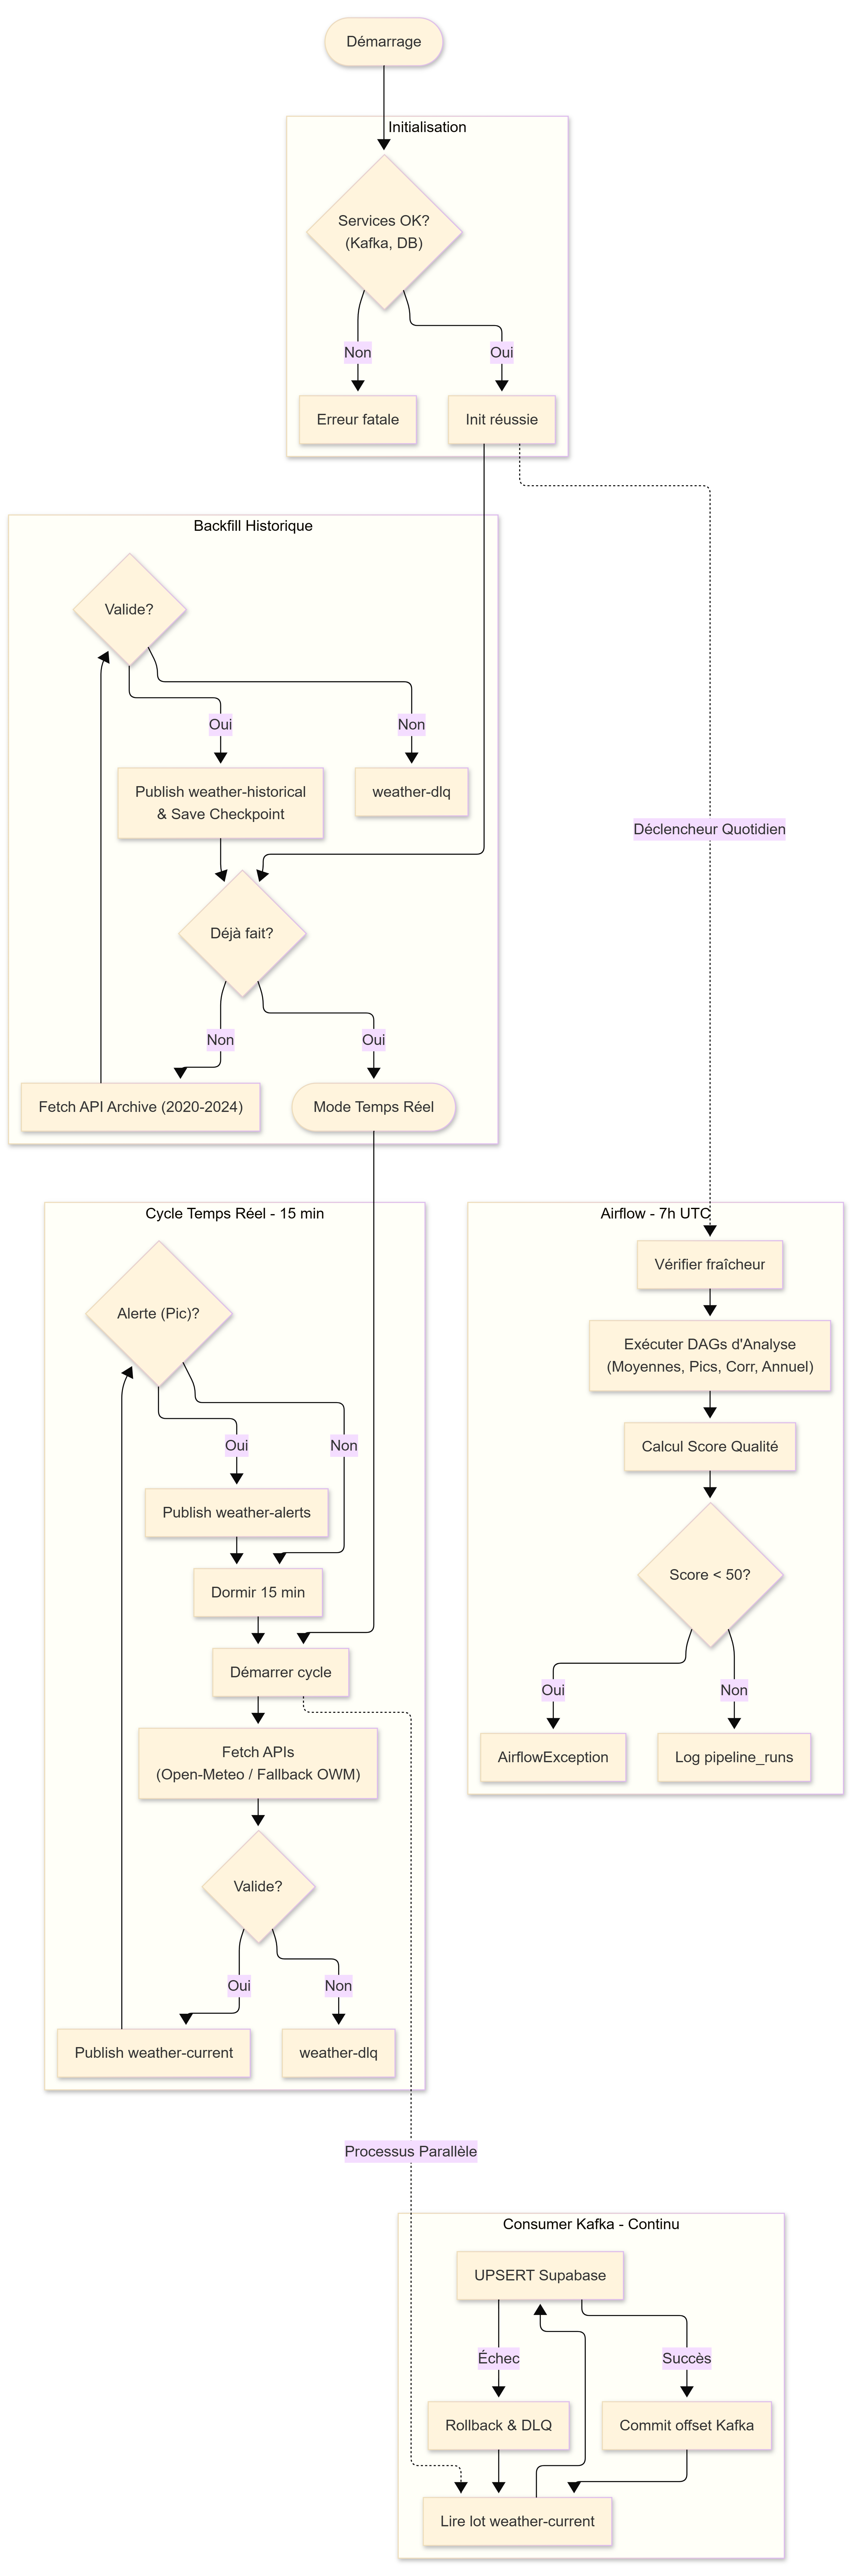
\includegraphics[width=\textwidth]{figures/activite.png}
\caption{Diagramme d'activité — Pipeline}
\end{figure}

\subsection{Diagramme de déploiement}
\begin{figure}[H]
\centering
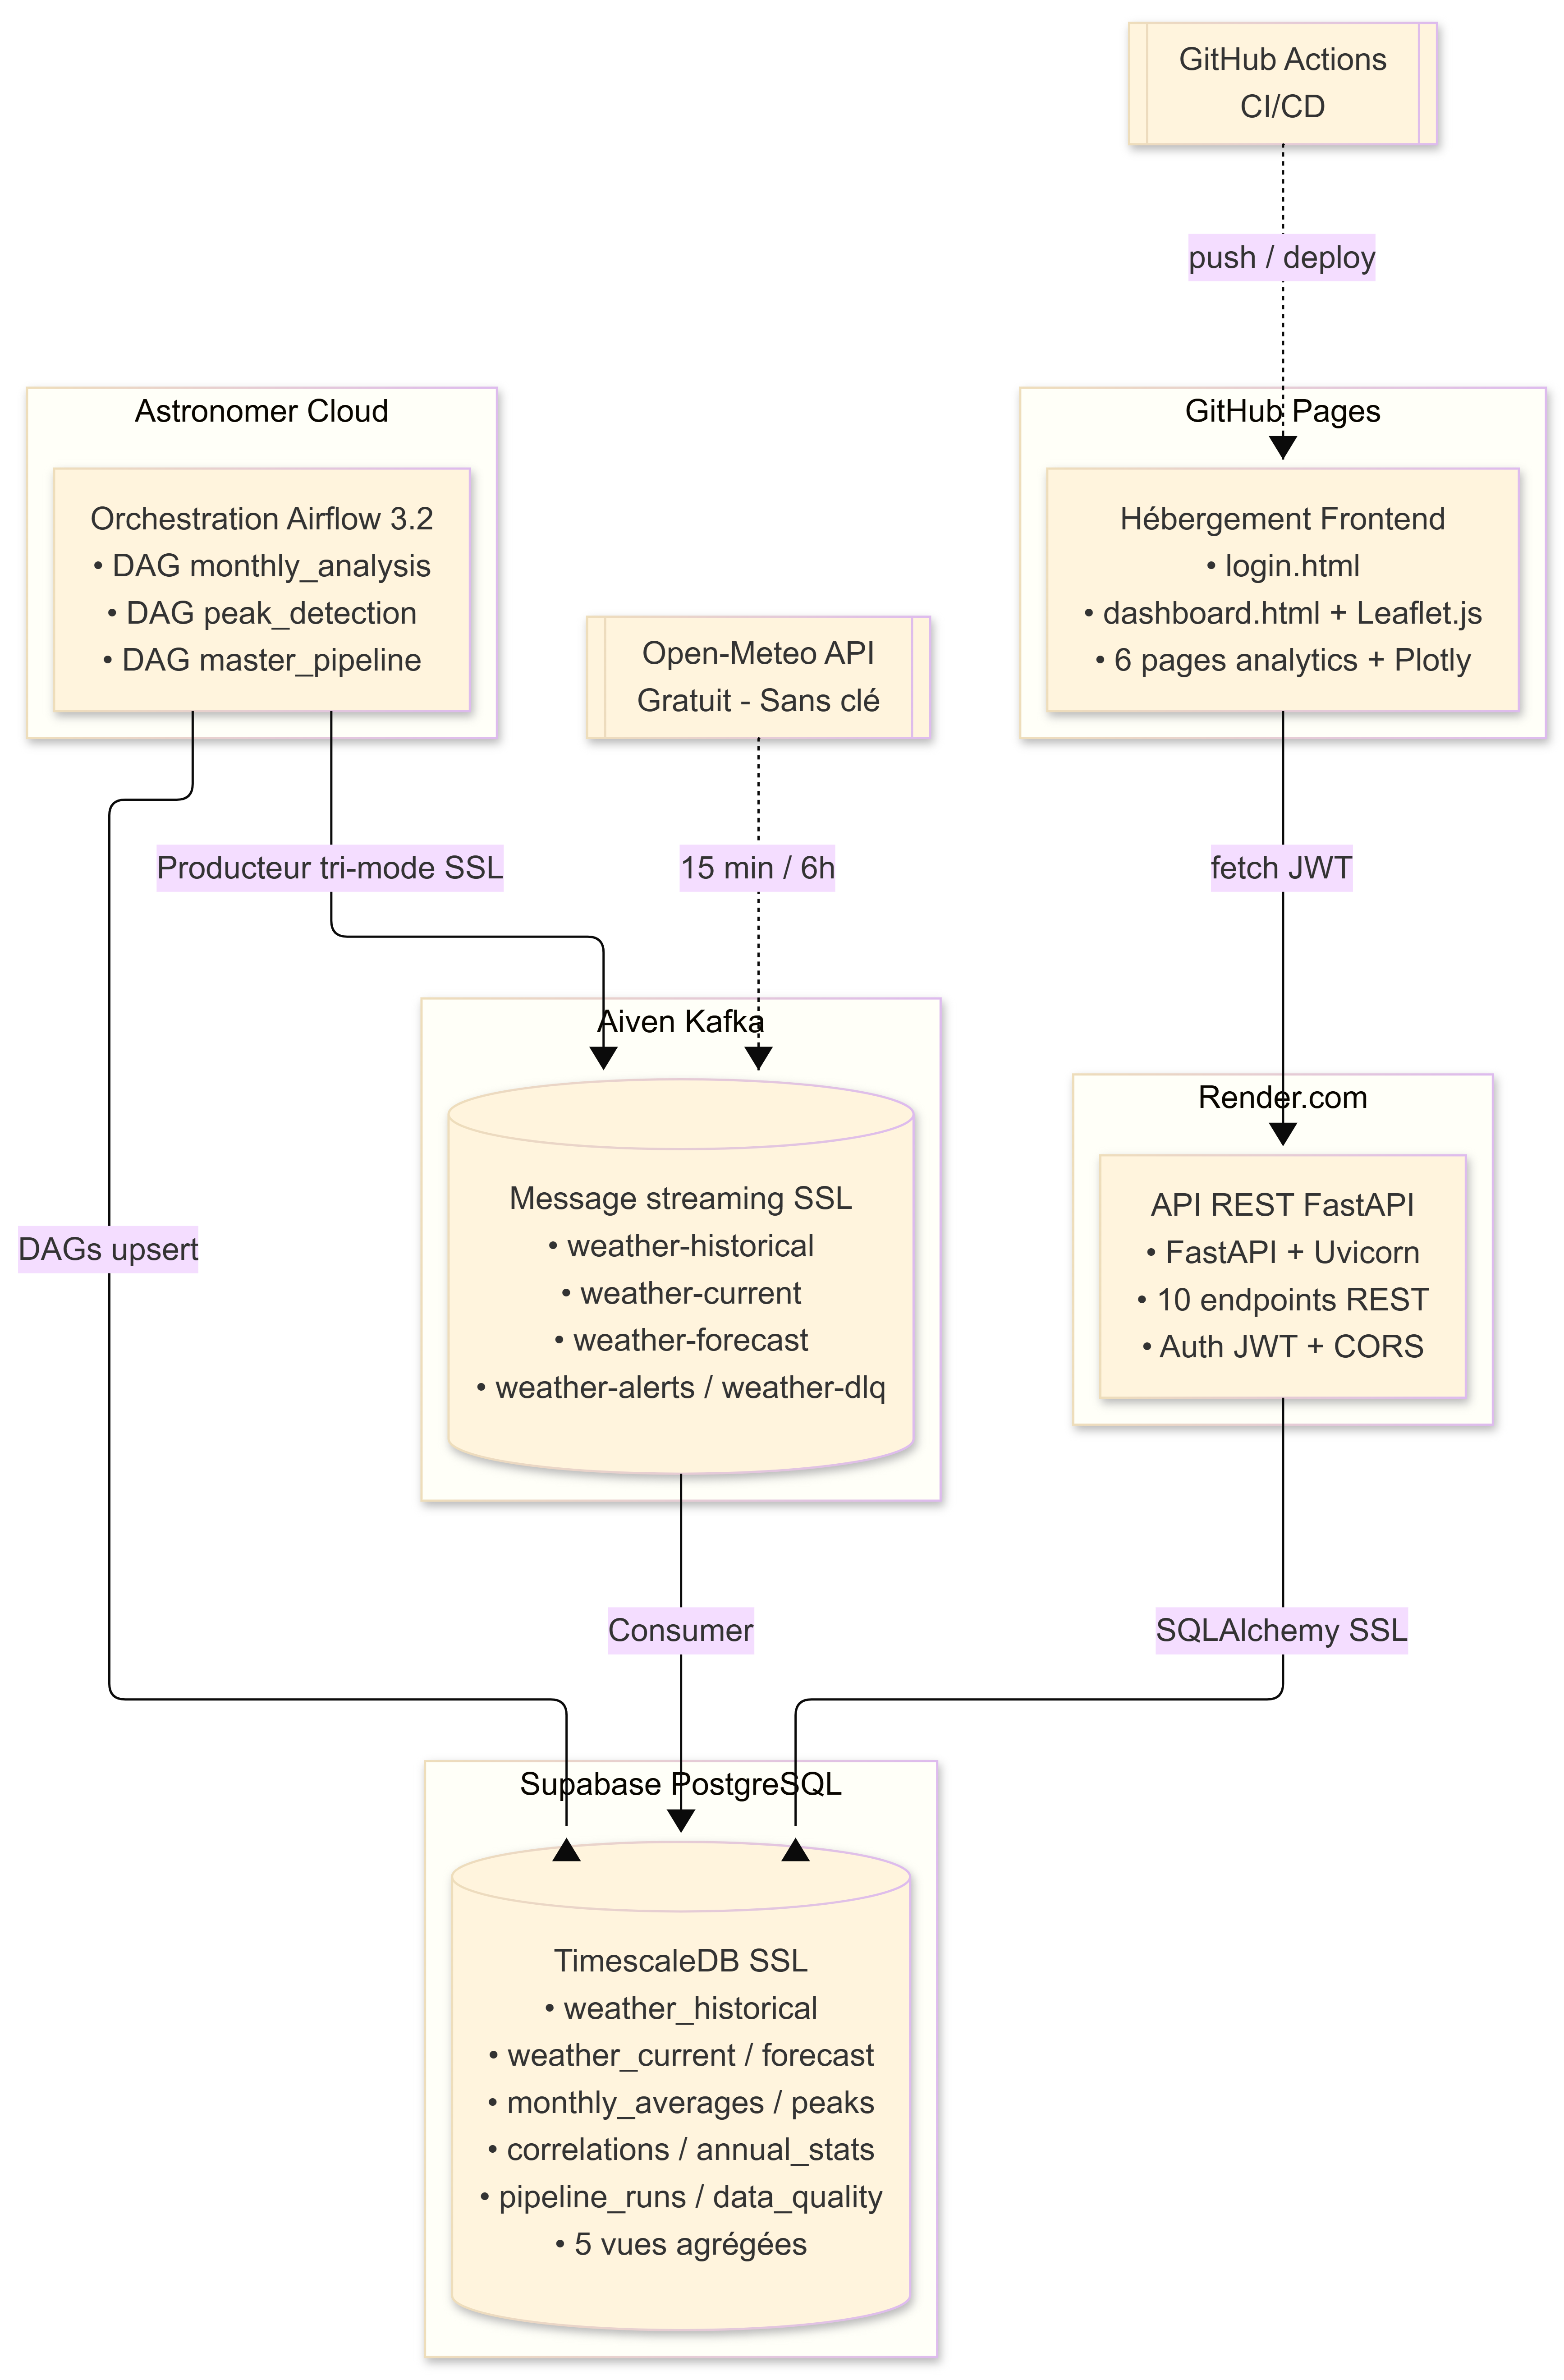
\includegraphics[width=\textwidth]{figures/deploiment.png}
\caption{Diagramme de déploiement}
\end{figure}

\section{Réalisation}
\subsection{Capture d'écran}
\begin{figure}[H]
\centering
\imgplaceholder{Figure~\ref{fig:airflow_ui}}{Capture de l'interface Airflow Astronomer}
\caption{Déploiement des DAGs sur l'environnement Cloud Airflow}
\end{figure}

\section{Tests et validations}
Les algorithmes statistiques développés ont été testés avec succès et l'orchestration avec Airflow fonctionne de manière 100\% automatisée sur le Cloud, respectant le planning d'exécution prévu.

\section{Conclusion}
Ce deuxième et dernier sprint finalise le projet. L'application est maintenant complète, fonctionnelle, déployée sur le Cloud, et répond parfaitement aux exigences techniques et fonctionnelles fixées dès le départ.

% CHAPITRE 6 — TESTS GLOBAUX
\chapter{Tests Globaux et Validation Finale}

\section{Stratégie globale de test}
La stratégie de test couvre quatre niveaux~: tests unitaires, tests d'intégration, tests de qualité des données et tests de performance. L'objectif est de garantir la fiabilité du pipeline de bout en bout.

\section{Tests unitaires consolidés (pytest)}

\begin{lstlisting}[language=bash,caption={Exécution des tests unitaires}]
$ pytest tests/ -v --cov=src --cov-report=term-missing
======================== 125 passed in 12.4s ========================
\end{lstlisting}

\begin{table}[H]\centering\caption{Couverture des tests unitaires}\label{tab:coverage}
\begin{tabularx}{\textwidth}{Xcccc}\toprule
\textbf{Module} & \textbf{Tests} & \textbf{Passés} & \textbf{Couverture} \\\midrule
\texttt{src/utils/db.py} & 12 & 12 & 89\% \\
\texttt{src/utils/cities.py} & 18 & 18 & 95\% \\
\texttt{src/utils/validator.py} & 15 & 15 & 92\% \\
\texttt{src/utils/kafka\_config.py} & 10 & 10 & 88\% \\
\texttt{src/producer.py} & 35 & 35 & 85\% \\
\texttt{src/consumer.py} & 20 & 20 & 82\% \\
\texttt{src/utils/weather\_codes.py} & 8 & 8 & 100\% \\
\midrule
\textbf{Total} & \textbf{125} & \textbf{125} & \textbf{87\%} \\\bottomrule
\end{tabularx}\end{table}

\begin{figure}[H]\centering
\imgplaceholder{Résultats pytest}{Capture d'écran du terminal montrant les 125 tests passés avec couverture}
\caption{Résultats des tests unitaires — pytest}\label{fig:pytest}\end{figure}

\section{Tests d'intégration (pipeline E2E)}
Le test d'intégration valide le flux complet~: Kafka $\rightarrow$ DB $\rightarrow$ API $\rightarrow$ Frontend.

\begin{table}[H]\centering\caption{Tests d'intégration E2E}\label{tab:e2e}
\begin{tabularx}{\textwidth}{clXc}\toprule
\textbf{ID} & \textbf{Flux} & \textbf{Description} & \textbf{OK} \\\midrule
E2E-01 & Historique & Producer envoie 221 villes $\rightarrow$ Consumer persiste $\rightarrow$ API retourne & \ding{51} \\
E2E-02 & Temps réel & OWM API $\rightarrow$ Kafka $\rightarrow$ DB $\rightarrow$ Dashboard refresh & \ding{51} \\
E2E-03 & Prévisions & Open-Meteo $\rightarrow$ Kafka $\rightarrow$ DB $\rightarrow$ /forecast endpoint & \ding{51} \\
E2E-04 & Analyses & Airflow DAG $\rightarrow$ Supabase $\rightarrow$ API $\rightarrow$ Plotly.js & \ding{51} \\\bottomrule
\end{tabularx}\end{table}

\section{Tests de qualité des données}
Le DAG \texttt{data\_quality\_monitor} vérifie quotidiennement~:
\begin{itemize}
  \item \textbf{Complétude}~: absence de valeurs NULL sur les champs critiques
  \item \textbf{Validité}~: température dans $[-5°C, 55°C]$
  \item \textbf{Unicité}~: absence de doublons (date, city)
  \item \textbf{Fraîcheur}~: dernière ingestion $< 48$h
\end{itemize}

\begin{figure}[H]\centering
\imgplaceholder{Quality scores}{Capture montrant les scores de qualité par couche (historical, current, forecast)}
\caption{Scores de qualité des données}\label{fig:quality}\end{figure}

\section{Tests de performance}

\begin{table}[H]\centering\caption{Métriques de performance}\label{tab:perf}
\begin{tabularx}{\textwidth}{Xlc}\toprule
\textbf{Métrique} & \textbf{Valeur mesurée} & \textbf{Objectif} \\\midrule
Ingestion historique (221 villes $\times$ 5 ans) & 25s & $<$ 60s \\
Ingestion temps réel (221 villes) & 8s & $<$ 30s \\
Exécution DAG monthly\_analysis & 12s & $<$ 60s \\
Exécution DAG peak\_detection & 18s & $<$ 60s \\
Latence API /summary & 120ms & $<$ 500ms \\
Chargement Dashboard & 1.2s & $<$ 3s \\\bottomrule
\end{tabularx}\end{table}

\section{Résultats et métriques — Bilan de vélocité}

\begin{table}[H]\centering\caption{Vélocité de l'équipe}\label{tab:velocity}
\begin{tabularx}{\textwidth}{Xccc}\toprule
\textbf{Sprint} & \textbf{Points planifiés} & \textbf{Points livrés} & \textbf{Vélocité} \\\midrule
Sprint 1 & 50 & 50 & 100\% \\
Sprint 2 & 26 & 26 & 100\% \\\midrule
\textbf{Total} & \textbf{76} & \textbf{76} & \textbf{100\%} \\\bottomrule
\end{tabularx}\end{table}

\begin{figure}[H]\centering
\imgplaceholder{Burndown chart}{Graphique burndown montrant la progression des deux sprints}
\caption{Burndown Chart — Sprints 1 et 2}\label{fig:burndown}\end{figure}


% ─────────────────────────────────────────
%  CONCLUSION
% ─────────────────────────────────────────
\chapter*{Conclusion et Perspectives}
\addcontentsline{toc}{chapter}{Conclusion et Perspectives}

\section*{Bilan du projet}
Au terme de ce projet, nous avons conçu et déployé une plateforme Big Data complète dédiée à la météorologie tunisienne. Le système couvre l'intégralité du cycle de vie de la donnée~: collecte depuis les APIs Open-Meteo et OpenWeatherMap, ingestion en temps réel via Apache Kafka (Aiven), stockage persistant sur Supabase (PostgreSQL), orchestration analytique via Apache Airflow déployé sur Astronomer Cloud, et visualisation interactive à travers un dashboard responsive.

Les principaux résultats incluent~:
\begin{itemize}
  \item Couverture de \textbf{221 villes tunisiennes} avec un historique de 5 ans (2020--2024).
  \item \textbf{6 DAGs Airflow} opérationnels~: analyses mensuelles, annuelles, détection de pics, corrélations saisonnières, qualité des données et pipeline maître.
  \item \textbf{125 tests unitaires} validant l'ensemble des modules.
  \item Un dashboard interactif avec thème sombre/clair et cartes Leaflet.js.
\end{itemize}

\section*{Limites et difficultés rencontrées}
\begin{itemize}
  \item La gestion des connexions IPv6 sur le tier gratuit de Supabase a nécessité le recours au Session Pooler.
  \item La synchronisation des certificats SSL Kafka entre l'environnement local et le conteneur Docker Astronomer.
  \item Le volume de données (221 villes $\times$ 5 ans $\times$ 4 variables) impose des optimisations SQL pour les analyses.
\end{itemize}

\section*{Perspectives d'amélioration}
\begin{itemize}
  \item Intégration de modèles de Machine Learning (LSTM, Prophet) pour la prévision météo.
  \item Ajout d'un système de notifications push (Firebase) pour les alertes météo critiques.
  \item Extension aux données satellite (Copernicus) pour une couverture spatiale plus fine.
  \item Migration vers TimescaleDB pour optimiser les requêtes temporelles.
\end{itemize}

% ─────────────────────────────────────────
%  BIBLIOGRAPHIE
% ─────────────────────────────────────────
\chapter*{Bibliographie}
\addcontentsline{toc}{chapter}{Bibliographie}

\begin{enumerate}[label={[\arabic*]}]
  \item Apache Software Foundation, \textit{Apache Kafka Documentation}, \url{https://kafka.apache.org/documentation/}, consulté en 2025.
  \item Apache Software Foundation, \textit{Apache Airflow Documentation}, \url{https://airflow.apache.org/docs/}, consulté en 2025.
  \item Supabase Inc., \textit{Supabase Documentation}, \url{https://supabase.com/docs}, consulté en 2025.
  \item Aiven Ltd., \textit{Aiven for Apache Kafka}, \url{https://aiven.io/kafka}, consulté en 2025.
  \item Open-Meteo, \textit{Free Weather API}, \url{https://open-meteo.com/}, consulté en 2025.
  \item Astronomer Inc., \textit{Astronomer Documentation}, \url{https://docs.astronomer.io/}, consulté en 2025.
  \item S.~Ramírez, \textit{FastAPI Documentation}, \url{https://fastapi.tiangolo.com/}, consulté en 2025.
  \item W.~McKinney, \textit{Python for Data Analysis}, O'Reilly Media, 3\textsuperscript{e} édition, 2022.
  \item K.~Schwaber et J.~Sutherland, \textit{The Scrum Guide}, 2020.
  \item M.~Kleppmann, \textit{Designing Data-Intensive Applications}, O'Reilly Media, 2017.
\end{enumerate}

% ─────────────────────────────────────────
%  ANNEXES
% ─────────────────────────────────────────
\appendix
\chapter{Schéma SQL Complet}
\label{app:sql}

\begin{lstlisting}[language=SQL,caption={Extrait du schéma de la base de données Supabase}]
-- Table principale des mesures historiques
CREATE TABLE weather_historical (
    id            SERIAL PRIMARY KEY,
    date          DATE NOT NULL,
    city          VARCHAR(100) NOT NULL,
    governorate   VARCHAR(100),
    region        VARCHAR(50),
    temperature   REAL,
    humidity      REAL,
    precipitation REAL,
    wind_speed    REAL,
    ingested_at   TIMESTAMPTZ DEFAULT NOW(),
    UNIQUE(date, city)
);

-- Table des moyennes mensuelles (calculee par Airflow)
CREATE TABLE monthly_averages (
    id            SERIAL PRIMARY KEY,
    year          INTEGER NOT NULL,
    month         INTEGER NOT NULL,
    city          VARCHAR(100) NOT NULL,
    governorate   VARCHAR(100),
    region        VARCHAR(50),
    avg_temp      REAL,
    max_temp      REAL,
    min_temp      REAL,
    avg_humidity  REAL,
    avg_precip    REAL,
    avg_wind      REAL,
    record_count  INTEGER,
    computed_at   TIMESTAMPTZ DEFAULT NOW(),
    UNIQUE(year, month, city)
);

-- Table des correlations saisonnieres
CREATE TABLE correlations (
    id              SERIAL PRIMARY KEY,
    variable_a      VARCHAR(50) NOT NULL,
    variable_b      VARCHAR(50) NOT NULL,
    season          VARCHAR(20) NOT NULL,
    pearson_r       REAL,
    p_value         REAL,
    interpretation  VARCHAR(50),
    is_significant  BOOLEAN,
    computed_at     TIMESTAMPTZ DEFAULT NOW(),
    UNIQUE(variable_a, variable_b, season)
);
\end{lstlisting}

\chapter{Configuration Kafka et Variables d'Environnement}
\label{app:config}

\begin{lstlisting}[caption={Fichier .env.example}]
# Aiven Kafka (SSL)
KAFKA_BOOTSTRAP=kafka-projetfedere-....aivencloud.com:21849
KAFKA_SECURITY_PROTOCOL=SSL
KAFKA_CA_FILE=ca.pem
KAFKA_CERT_FILE=service.cert
KAFKA_KEY_FILE=service.key

# Supabase PostgreSQL
DB_HOST=aws-1-eu-central-1.pooler.supabase.com
DB_PORT=5432
DB_NAME=postgres
DB_USER=postgres.your_project_ref
DB_PASSWORD=your_password

# Weather APIs
TIMEZONE=Africa/Tunis
START_DATE=2020-01-01
END_DATE=2024-12-31
OWM_API_KEY=your_api_key
\end{lstlisting}

\chapter{Guide de Déploiement}
\label{app:deploy}

\section{Supabase}
\begin{enumerate}
  \item Créer un projet sur \url{https://supabase.com}
  \item Exécuter le schéma SQL (Annexe~\ref{app:sql}) dans l'éditeur SQL
  \item Récupérer le host du Session Pooler (Settings $\rightarrow$ Database)
\end{enumerate}

\section{Aiven Kafka}
\begin{enumerate}
  \item Créer un service Kafka sur \url{https://aiven.io}
  \item Télécharger les certificats SSL (ca.pem, service.cert, service.key)
  \item Créer les topics~: \texttt{weather-historical}, \texttt{weather-current}, \texttt{weather-forecast}
\end{enumerate}

\section{Astronomer Cloud (Airflow)}
\begin{enumerate}
  \item Installer Docker Desktop et le CLI Astro~: \texttt{brew install astro}
  \item Se connecter~: \texttt{astro login}
  \item Valider les DAGs~: \texttt{astro dev parse}
  \item Déployer~: \texttt{astro deploy}
  \item Configurer les variables d'environnement dans l'UI Astronomer
\end{enumerate}

\chapter{Manuel Utilisateur}
\label{app:user}

\section{Accès au Dashboard}
L'utilisateur accède à la plateforme via un navigateur web. La page d'accueil présente un tableau de bord avec les indicateurs météo principaux.

\imgplaceholder{Figure — Dashboard principal}{Capture d'écran du dashboard avec les KPIs météo, la carte Leaflet et les graphiques Plotly.js}

\section{Navigation}
\begin{itemize}
  \item \textbf{Accueil}~: Vue d'ensemble avec carte interactive
  \item \textbf{Temps réel}~: Données actuelles avec rafraîchissement automatique
  \item \textbf{Prévisions}~: Prévisions à 7 jours par ville
  \item \textbf{Analyses}~: Corrélations, tendances annuelles, pics thermiques
\end{itemize}

\end{document}
